%!TEX root = ../template.tex
%%%%%%%%%%%%%%%%%%%%%%%%%%%%%%%%%%%%%%%%%%%%%%%%%%%%%%%%%%%%%%%%%%%
%% chapter1.tex
%% NOVA thesis document file
%%
%% Chapter with introduciton
%%%%%%%%%%%%%%%%%%%%%%%%%%%%%%%%%%%%%%%%%%%%%%%%%%%%%%%%%%%%%%%%%%%


\chapter{Methodologies}
\label{cha:methodologies}
Taking into account the existing usability problems and the target users' requirements and expectations, a methodology is essential to design, implement, and evaluate solutions throughout the development process. Therefore, this chapter presents the approached phases and techniques across the solution conception, from the first sketches to the final evaluations. 

\section{Iterative Design}
\label{sec:iterative_design}
Before starting the solution building process, it was planned the phases that will conduct the development to the final solution of this dissertation. Accordingly, it is presented the design strategy adopted, which will be further detailed in \nameref{cha:design_and_implementation}. This methodology uses an iterative design strategy in order to keep a user-centric design, which prioritizes the users' needs according to the mentioned in \ref{subsec:user_centered_design}. Regarding the prototyping method, the evolutionary prototyping principle (described in \ref{subsubsec:sketching_and_prototyping}) was applied, where the last prototype is used as a baseline to develop the prototype of the next iteration.

\textbf{Sketching: }The design process started with an initial sketching phase, where the first solution ideas were explored and crafted. This is a favorable technique to contemplate how new ideas could be integrated into the existing interface. The most important aspect was to think about system transversal changes and not about particular details of specific components, since these details could be refined later. The outcome of this phase should set a more concrete idea in what can be inserted in the prototype, even if it is necessary to think more about how to implement it later.

Keeping in mind these concrete ideas explored, it was possible to start to build the prototypes that want to be tested by users. The first decision taken was how many prototypes should be built taking into consideration the resources and time available. As mentioned in \ref{subsubsec:sketching_and_prototyping}, the first prototypes should be low-fidelity prototypes and iteration by iteration this level should increase in order to refine details in the interface. In that way, it was decided to built two prototypes:

%Therefore, the following phases presented were used to iteratively build the solution which took into account the users adoption at the final of each iteration:

\begin{itemize}
    \item \textbf{Paper Prototype: } Simple low-fidelity prototype implemented in paper using ruler, square, and writing materials. By this approach, it was possible to implement the first ideas faster and with a low-risk. The main concern of this prototype is the design of the major interface changes, not only in terms of layout but also the changes that might affect users' mental model. In that way, it was possible to evaluate early if the design choices applied should continue to the next iterations or if they should be redesigned.
    \item \textbf{Service Studio Prototype: } This is the final prototype of this dissertation, that was developed using C\#, Typescript \cite{typescript}, and React \cite{react}, and integrated in the new Design of Service Studio. Through this prototype, the solutions implemented were validated and compared with the previous existing implementation in order to validate if the usability of the system proposed has improved.
\end{itemize}

In each one of the two above-mentioned prototypes, it was included the following phases: design, implementation, and evaluation. The Design phase was where it was thought how the solution ideas could be applied. The Implementation phase refers to the concrete prototype development process. Finally, in the Evaluation phase the prototypes were tested by final users, according to the testing approach explained below in \ref{sec:testing_scenarios} and \ref{sec:evaluation_method}.

Regarding evaluation, it was necessary to establish how many users should be tested in each one of the evaluating phases. Nevertheless, these two prototypes were not the only ones tested by final users, since the existing implementation was already tested in order to evaluate the current problems of the system. The data of that analysis is also an opportunity to has a baseline of the development starting point across the solution building. Thereby, the number of users tested in the first prototype is also an important factor.

Nielsen performed some studies to quantify how many users should be testing in a usability study, concluding that 5 users are sufficient for qualitative studies because it is almost possible to get close to the user testing's maximum benefit-cost ratio - "Testing with 5 people lets you find almost as many usability problems as you'd find using many more test participants" \cite{why_you_only_need_to_test_with_5_users} \cite{how_many_test_users_in_a_usability_study}. However, to perform quantitative analysis it is necessary to get at least 20 users in order to get statistical relevance \cite{how_many_test_users_in_a_usability_study}.

According to the studies mentioned, at least 5 users of each user group (described in \ref{sec:target_users}.) should be tested since it would be performed a qualitative analysis to validate how users react to the changes applied and what could be improved in the next phase. Nevertheless, some statistical results should be also retrieved in order to compare in other aspects if the new solution provides improved usability than the existing with the previous one. Hence, it was been tested more users in the previous implementation and in the final prototype in order to obtain also quantitative comparisons. In that way, Table \ref{tab:number_of_users_tested_by_each_user_group_and_solution} shows how many users were tested by each user group and by each solution evaluated.

\begin{table}[tb]
	\caption{Number of users tested by each user group and by each solution evaluated}
	\label{tab:number_of_users_tested_by_each_user_group_and_solution}
\centering
\resizebox{\textwidth}{!}{
\begin{tabular}{c|c|c|c|c|}
    \cline{2-5}
    \rowcolor[HTML]{C0C0C0} 
    \cellcolor[HTML]{FFFFFF}                                 & Previous Implementation & Paper Prototype & Service Studio Prototype & Total \\ \hline
    \multicolumn{1}{|c|}{\cellcolor[HTML]{C0C0C0}OutSystems Developer}    & 10         & 5               & 10                    & 25 \\ \hline
    \multicolumn{1}{|c|}{\cellcolor[HTML]{C0C0C0}Software Developer} & 10        & 5              & 10                   & 25\ \\ \hline
    \multicolumn{1}{|c|}{\cellcolor[HTML]{C0C0C0}Citizen Developer} & 10        & 5              & 10                   & 25\ \\ \hline
    \multicolumn{1}{|c|}{\cellcolor[HTML]{C0C0C0}Total} & \textbf{30}        & \textbf{15}              & \textbf{30}                   & \textbf{75}\ \\ \hline
    \end{tabular}
    }
\end{table}


\section{Testing Scenarios}
\label{sec:testing_scenarios}
Given the wide scope of the usability problems identified, there was a necessity to plan a testing approach that could evaluate the most important aspects of the user-interface communication in a short period. Otherwise, each user test would have a longer duration which would not be affordable.

The first point defined was the type of testing scenarios that would be proposed. For that decision, it was taken into account what were the specific aspects that should be improved in the interface usability. As mentioned, not only the optimization of the efficiency, effectiveness, learnability, and user satisfaction of the entire query formulation process was the goal, but also the improvement of the query comprehension. In such a way that it was important to evaluate if users could understand the query purpose (i.e., what data intends to be fetched from the database) as well as the time they required to realize that.

Considering those evaluation requirements, two types of testing scenarios were prepared: scenarios where users explore an existing query built through the visual querying tool and try to realize what is its purpose, and the other ones where users try to formulate it on their own. Through that approach, it was possible to analyze the usability of the interfaces tested for both points of view: comprehension and formulation.

Nevertheless, the complexity of the queries presented acts as a crucial factor when the scenarios were thought out. For example, an interface could be useful and pleasant to use in simple use cases but it could not keep that quality in more complex queries. Accordingly, there was listed the requirements that were considered relevant to be covered by user testing scenarios:

\begin{itemize}
    \item \textbf{Query Comprehension: }Relevant aspects which should be present in the queries and consequently in the interface to evaluate as extensive as possible queries' comprehension:
    \begin{itemize}
        \item \textbf{Interface Elements Exploration: }Include use cases that contain the majority of the query components supported by the system: database entities and joins of different types, filtering and sorting criteria applied to different data types, and other query components added throughout the query formulation process, such as Group Bys, Aggregation Functions (SUM, MIN, MAX, AVG, COUNT) or Calculated Attributes \footnote{These operations were presented in \ref{subsubsec:current_progress}};
        \item \textbf{Joins Representation: }Representation of different joins in order to analyze if users could successfully identify them. First of all, there was the concert to consider in scenarios joins of different types, such as inner joins or left joins. In addition, the natural joins (i.e., joins where the unique foreign key that references the other table is equals to the other table primary key) were not the only considered. Besides these joins, some queries that contain joins with more advanced conditions were also covered. For instance, when the join between two tables could be made using different foreign keys, as they are multiple relationships between both tables, or when the join condition contains logical operators.
    \end{itemize}
    \item \textbf{Query Formulation: }At the same time, the following aspects were considered essential to be approached in user testing scenarios from a query formulation point of view:
    \begin{itemize}
        \item \textbf{Add Data Sources and Joins: }Identify the options chosen to add query sources and analyze what are the users' reactions to the system automatisms to simplify the joins specification;
        \item \textbf{Edit Query Filters: }Evaluate if the query filters edition is intuitive and what barriers could exist in the interfaces regarding this aspect;
        \item \textbf{Insert Calculated Attributes, Group Bys, and Aggregation Functions: }Check if users could understand the situations they need to use each on of the referred functionalities and if they can discover how to apply them without difficulty.
        \item \textbf{Use Hidden Columns: }Verify the difficulty felt by users when they need to apply actions in attributes that are not always visible in the interface, either because they are hidden, or because they are not visible due to the lack of available space in the interface (scroll required).
    \end{itemize}
\end{itemize}

The aspects mentioned were considered the most relevant to analyze because they allow widespread use of the tool but also cover cases identified as critical in terms of usability, according to the aspects detailed in \ref{sec:problem_definition}.

Nevertheless, the data model could have also a significant impact on user testing results. For instance, if a user does not understand a data model, he could not realize the purpose of a query, even if the query is presented in a simple and readable manner. In that way, the selection of the data model used for user testing was performed attending to the following points:

\begin{itemize}
    \item \textbf{Simple Business Domain: }If the purpose of the database is to store and manage data that has a simple and practical day-to-day application, it would be simple to understand the data model regardless of the user's background;
    \item \textbf{Different data types: }A data model that contains a variety of data types it would be useful to analyze if the design approaches chosen could work for all types;
    \item \textbf{Multiple relationships between two entities: }The interface aims to accelerate and simplify the querying process not only for simple cases. For this reason, it is important to perceive how the interface could support users in cases that there are more than one relationship between two entities. Moreover, \gls{SQL} does not have any particular syntax that helps users in these cases, then there is an improvement opportunity here.
\end{itemize}

\begin{figure}[htbp]
	\centering
	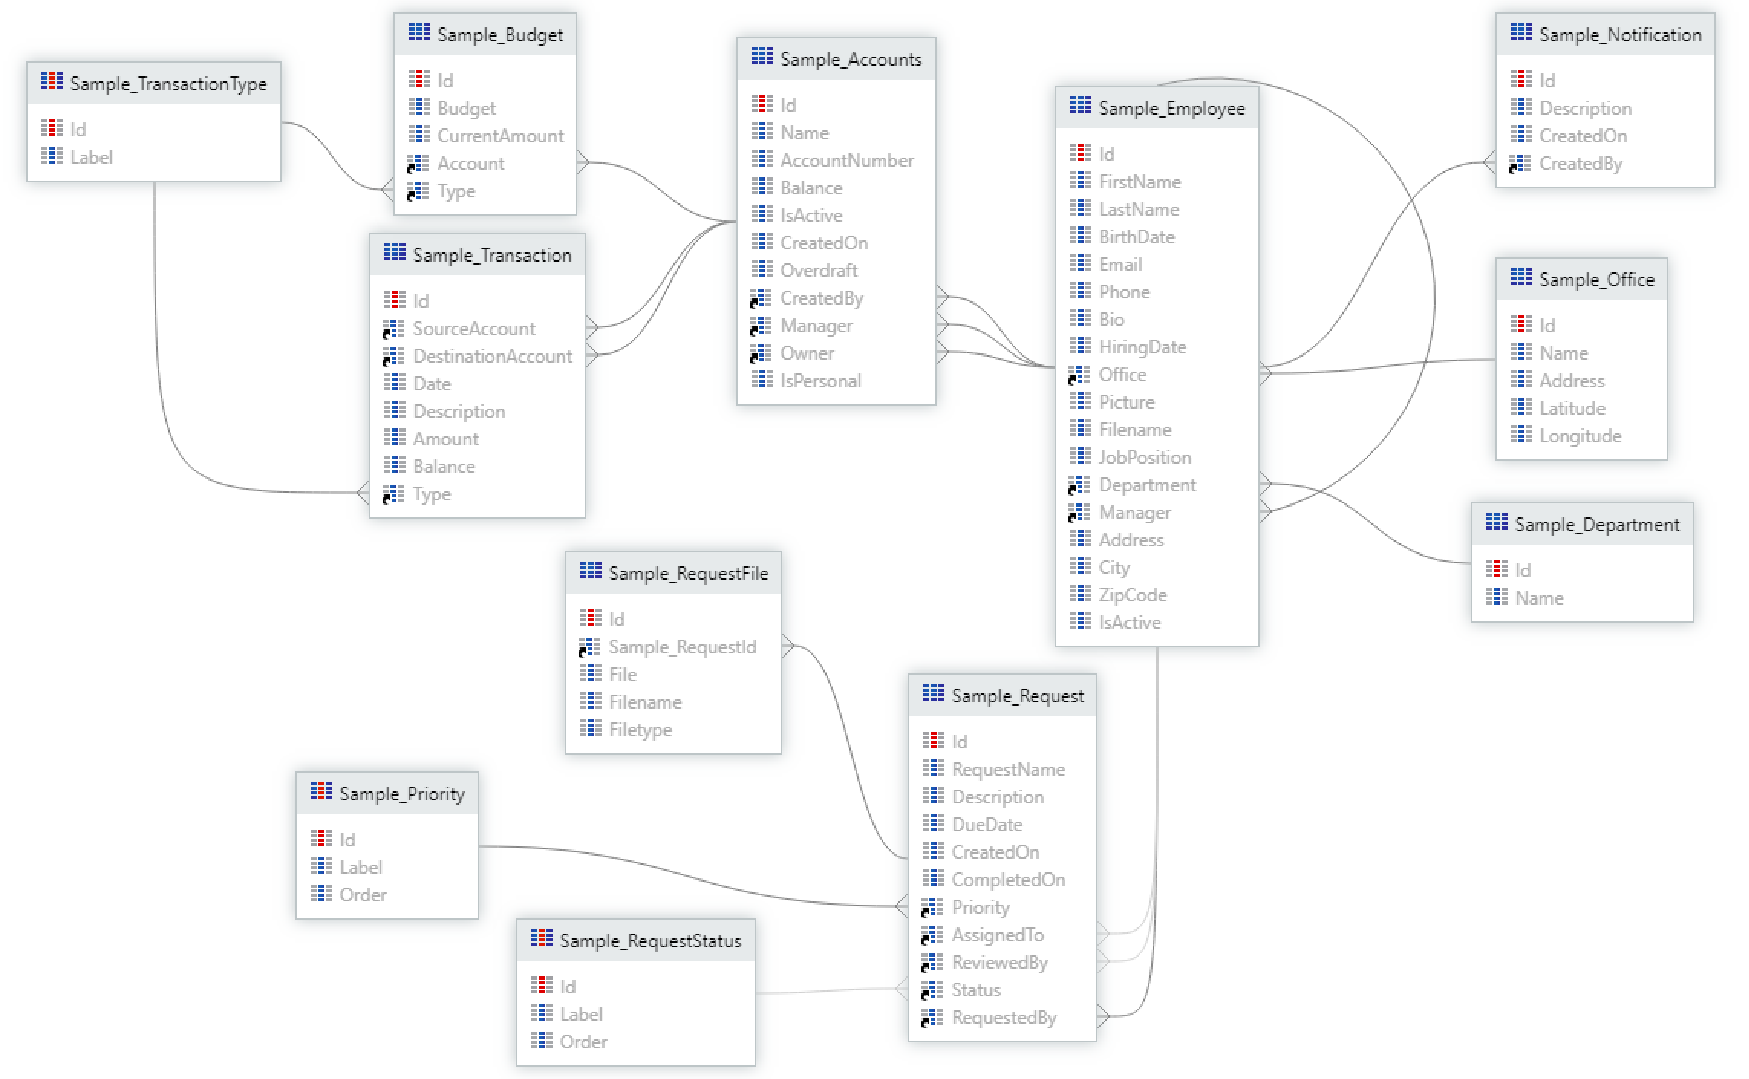
\includegraphics[height=3.6in]{data-model}
	\caption{Data Model used for User Testing}
	\label{fig:dataModel}
\end{figure}

Accordingly, \ref{fig:dataModel} illustrates the data model of the database adopted to perform all usability tests.

After choosing the data model used as support for the usability tests, the list of test scenarios was elaborated. There were designed three different types of scenarios:

\begin{itemize}
    \item \textbf{Query Comprehension: } The user explores a visual query already built and tries to indicate what are the query components presented as well as the data that would be fetched from the database through that query;
    \item \textbf{Query Modification: } After a query comprehension example, the user tries to apply some modification on the existing query previously explored;
    \item \textbf{Query Formulation: } Given a natural language statement that explains what data is intended to be fetched from the database, the user tries to retrieve them formulating a new visual query from scratch.
\end{itemize}

Through that approach, it was possible to keep the focus on different aspects according to the scenario used. On the one hand, the comprehension scenarios gives the focus to the query readability, which promote a global exploration of the query components and gave the opportunity to understand if users clearly indentified the purpose of each interface section. On the other hand, modification and formulation scenarios were used to understand if users could built queries through the interface presented.

Nevertheless, there was several results to be obtained from the user testing scenarios and it was difficult reach an approach to test all aspects related to the existing problems in a short period. Since the testing requirements presented above must be integrated in the scenarios, a strategy was used to distribute the different requirements among the different scenarios in order to evaluate them all in a fluid and natural way for the user. 

%Considering the short period available to test all mentioned requirements, the aspects considered essential to be present in the use cases explored were combined in a table in order to distribute them along a set of scenarios. Figure X 

Therefore, Table \ref{tab:scenarios_complexity} was used to assign organize the complex of each scenarios and check what aspects would e tested in each one.

\textbf{Table \ref{tab:scenarios_complexity} clarifications regarding the factors integrated in testing scenarios: }
\begin{itemize}
    \item \textbf{Simple Joins: }Joins that are automatically generated by the system without requiring human intervention;
    \item \textbf{Complex Joins: }Joins that need to be parcially configured manually (e.g., to specify the foreign key used to merge both tables or to change the join condition);
    \item \textbf{Left Join with Null: }Left join between entities A and B, to consider only the entities A that are not related to B (e.g., the employees who have not created any notification.);
    \item \textbf{Group by (without reference): } The system has an automatism that generates automatically a name to a new attribute grouped by. However, this name is not self explanatory and there was no reference to the source of its attribute. That way, it is important to highlight this case;
    \item \textbf{Aggregation Functions: } The aggregation functions supported by aggregates are Max, Min, Average, Sum, and Count. As the representation in the interface as well as the insertion method is similar, only a few of these were used;
\end{itemize}

\begin{table}[tb]
    \caption{Distribution of the relevant testing aspects among the testing scenarios designed.}
	\label{tab:scenarios_complexity}
    \begin{tabular}{|l|l|c|c|c|c|c|c|c|}
        \hline
        \multicolumn{2}{|l|}{\textbf{Scenarios}}                                                                                                                                                          & \multicolumn{1}{l|}{\textbf{C1}}           & \multicolumn{1}{l|}{\textbf{M1}} & \multicolumn{1}{l|}{\textbf{C2}}           & \multicolumn{1}{l|}{\textbf{C3}}           & \multicolumn{1}{l|}{\textbf{F1}} & \multicolumn{1}{l|}{\textbf{C4}}           & \multicolumn{1}{l|}{\textbf{M4}} \\ \hline
                                                                                                                               & Number of Entities                                                       & 4                                          & 4                                & 6                                          & 3                                          & 3                                & 5                                          & 7                                \\ \cline{2-9} 
                                                                                                                               & Simple Joins                                                             & 2                                          & 2                                & 4                                          & 2                                          & 1                                & 3                                          & 3                                \\ \cline{2-9} 
                                                                                                                               & Complex Joins                                                            & -                                          & -                                & 1                                          & -                                          & 1                                & 1                                          & 3                                \\ \cline{2-9} 
                                                                                                                               & Left Join with Null                                                      & 1                                          & 1                                & -                                          & -                                          & -                                & -                                          & -                                \\ \cline{2-9} 
                                                                                                                               & Filters                                                                  & 3                                          & 2                                & 3                                          & -                                          & -                                & 1                                          & 2                                \\ \cline{2-9} 
                                                                                                                               & Group Filters                                                            & -                                          & -                                & -                                          & -                                          & 1                                & -                                          & -                                \\ \cline{2-9} 
                                                                                                                               & Sorting (Text)                                                           & 1                                          & 1                                & -                                          & -                                          & -                                & 1                                          & 1                                \\ \cline{2-9} 
                                                                                                                               & Sorting (Number)                                                         & -                                          & -                                & 1                                          & 1                                          & -                                & -                                          & -                                \\ \cline{2-9} 
                                                                                                                               & Sorting (Date)                                                           & -                                          & -                                & -                                          & -                                          & -                                & 1                                          & 1                                \\ \cline{2-9} 
                                                                                                                               & Group By                                                                 & -                                          & -                                & 1                                          & 2                                          & 4                                & -                                          & -                                \\ \cline{2-9} 
                                                                                                                               & \begin{tabular}[c]{@{}l@{}}Group By \\ (without reference)\end{tabular}  & -                                          & -                                & -                                          & 3                                          & -                                & -                                          & -                                \\ \cline{2-9} 
                                                                                                                               & Max                                                                      & -                                          & -                                & -                                          & -                                          & -                                & -                                          & -                                \\ \cline{2-9} 
                                                                                                                               & Min                                                                      & -                                          & -                                & -                                          & -                                          & -                                & -                                          & -                                \\ \cline{2-9} 
                                                                                                                               & Average                                                                  & -                                          & -                                & -                                          & -                                          & 1                                & -                                          & -                                \\ \cline{2-9} 
                                                                                                                               & Sum                                                                      & -                                          & -                                & 1                                          & -                                          & -                                & -                                          & -                                \\ \cline{2-9} 
        \multirow{-16}{*}{\textbf{\begin{tabular}[c]{@{}l@{}}Relevant for\\ Comprehension\\ and Formulation\end{tabular}}}     & Count                                                                    & -                                          & -                                & -                                          & 1                                          & -                                & -                                          & -                                \\ \hline
                                                                                                                               & \begin{tabular}[c]{@{}l@{}}Use of not \\ visible columns\end{tabular}    & \cellcolor[HTML]{EFEFEF}                   &                                  & \cellcolor[HTML]{EFEFEF}                   & \cellcolor[HTML]{EFEFEF}                   & X                                & \cellcolor[HTML]{EFEFEF}                   &                                  \\ \cline{2-2} \cline{4-4} \cline{7-7} \cline{9-9} 
                                                                                                                               & \begin{tabular}[c]{@{}l@{}}Use of hidden \\ columns\end{tabular}         & \cellcolor[HTML]{EFEFEF}                   &                                  & \cellcolor[HTML]{EFEFEF}                   & \cellcolor[HTML]{EFEFEF}                   & X                                & \cellcolor[HTML]{EFEFEF}                   &                                  \\ \cline{2-2} \cline{4-4} \cline{7-7} \cline{9-9} 
                                                                                                                               & \begin{tabular}[c]{@{}l@{}}Insert \\ Calculated Attribute\end{tabular}   & \cellcolor[HTML]{EFEFEF}                   & X                                & \cellcolor[HTML]{EFEFEF}                   & \cellcolor[HTML]{EFEFEF}                   &                                  & \cellcolor[HTML]{EFEFEF}                   &                                  \\ \cline{2-2} \cline{4-4} \cline{7-7} \cline{9-9} 
                                                                                                                               & \begin{tabular}[c]{@{}l@{}}Add \\ Aggregation Function\end{tabular}      & \cellcolor[HTML]{EFEFEF}                   &                                  & \cellcolor[HTML]{EFEFEF}                   & \cellcolor[HTML]{EFEFEF}                   & X                                & \cellcolor[HTML]{EFEFEF}                   &                                  \\ \cline{2-2} \cline{4-4} \cline{7-7} \cline{9-9} 
                                                                                                                               & \begin{tabular}[c]{@{}l@{}}Add not \\ automatic join\end{tabular}        & \cellcolor[HTML]{EFEFEF}                   &                                  & \cellcolor[HTML]{EFEFEF}                   & \cellcolor[HTML]{EFEFEF}                   & X                                & \cellcolor[HTML]{EFEFEF}                   & X                                \\ \cline{2-2} \cline{4-4} \cline{7-7} \cline{9-9} 
                                                                                                                               & \begin{tabular}[c]{@{}l@{}}Add same entity \\ twice (alias)\end{tabular} & \cellcolor[HTML]{EFEFEF}                   &                                  & \cellcolor[HTML]{EFEFEF}                   & \cellcolor[HTML]{EFEFEF}                   &                                  & \cellcolor[HTML]{EFEFEF}                   & X                                \\ \cline{2-2} \cline{4-4} \cline{7-7} \cline{9-9} 
        \multirow{-7}{*}{\textbf{\begin{tabular}[c]{@{}l@{}}Relevant for \\ Query Formulation\\ or Modification\end{tabular}}} & Edit some filters                                                        & \multirow{-7}{*}{\cellcolor[HTML]{EFEFEF}} & X                                & \multirow{-7}{*}{\cellcolor[HTML]{EFEFEF}} & \multirow{-7}{*}{\cellcolor[HTML]{EFEFEF}} &                                  & \multirow{-7}{*}{\cellcolor[HTML]{EFEFEF}} &                                  \\ \hline
        \end{tabular}
    \end{table}


All scenarios are detailed in \nameref{app:user_testing_scenarios}, including for each scenario, the description of the testing scenario proposed and the main points taken into account throughout the tests performed.

%\textbf{User Testing Scenarios:}
%Accordingly, there were created the following test scenarios in order to evaluate the usability of the system, taking also into account the aspects more relevant above mentioned:

%In order to built scenarios that not only have different complexity levels but also approach the aspects that should be tested, there 
\section{Evaluation Method}
\label{sec:evaluation_method}
Having all testing scenarios established, it was necessary to plan how to identify the user, evaluate its interaction with the system, and collect qualitative and quantitative results throughout the usability tests.

First of all, users filled a survey in order to perceive what are their background regarding software development, relational databases, and data management and visualization tools. The answers were used to realize what are the their user profile according to the user groups defined in \ref{subsec:user_groups}.

After perceiving what are the most appropriate user group for the user in question, the data model is presented focusing the most relevant aspects for the tests. In that way, it is explained how the entities of the model are related with each other and the attributes most used in scenarios are highlighted.

As soon as they confirme that they got an overview of the existing entities, the testing process starts. However, following users reasoning and opinions while they interacs with with the interface was not considered sufficient to collect all results necessary.

Therefore, an evaluation methodology was designed to collect 